\chapter{Experiments and Results}

In this section a description of the experiment is defined, followed by the experimental results. 

\section{Description of Experiment}
\label{sec:experiment}
To experiment with different solutions for sentiment analysis, a system testing platform and code base was developed. This testing system generates and trains different models based on input arguments as default values for algorithms and type of algorithm. The architecture and flow of this system is described as a part of section~\ref{sec:classifier_arch}.

The testing system can take in a set of parameters to use for an algorithm, like pre-processor methods, whether or not to use inverse document frequency (\nom{IDF}{Inverse Document Frequency}) or stop words and so on, or a grid search flag can be set. If the grid search option is activated, a model is generated with the best possible parameters set for the given algorithm. The grid search is conducted using k-fold cross validation, and the set of parameters to search across. The parameter search space is reflected in table~\ref{tab:gridsearch_params}.


\begin{table}[!htb]
\centering
\begin{tabular}{|r||c|c|c|} 
\cline{2-4}

\multicolumn{1}{c|}{ } & \textbf{NB} & \textbf{SVM} & \textbf{MaxEnt} \\ \hline

penalty  &  - &  - & L1 or L2 \\ \hline
alpha/C  & \multicolumn{3}{ c| }{<0.1, 0.3, 0.5, 0.7, 0.8, 1.0>} \\ \hline
ngram &  \multicolumn{3}{ c| }{ Unigram, Bigram or Trigram } \\ \hline
Remove Stop Words &  \multicolumn{3}{ c| }{ Yes or No } \\ \hline
Use IDF &  \multicolumn{3}{ c| }{ Yes or No } \\ \hline
Use Smooth IDF &  \multicolumn{3}{ c| }{ Yes or No } \\ \hline
Use Sublinear IDF &  \multicolumn{3}{ c| }{ Yes or No } \\ \hline

\end{tabular}
\caption{Overview of parameter search space for the grid searches conducted in the experiments.}
\label{tab:gridsearch_params}
\end{table}

\subsection{Pre-processing and Feature Selection}

This section describes the different pre-processing implementations used; what placeholders, negation attachment and reducing letter duplications is.

To find the best features to use and what kind of pre-processing was the best, a set of 8 different combination of pre-processing methods was designed. The different methods include no pre-processing, where all characters are included as features, full remove where all special Twitter features like user names, URLs, hash tags and emoticons are stripped and one where the Twitter features are replaced with placeholder texts to reduce vocabulary. A full view of the pre-processing methods can be viewed in~table~\ref{tab:preproc_desc}.

\begin{table}[!htb]
	\centering
	\begin{tabular}{|r||c|c|c|c|c|c|c|c|}
		% P1  -> no\_usernames
		% P2 -> remove\_noise
		% P3 -> placeholders
		% P4 -> all
		% P5 -> remove\_all
		% P6 -> reduced\_attached
		% P7 -> no\_url\_usernames \_reduced \_attached

		\cline{2-9}
	 \multicolumn{1}{c| }{ } & \textbf{None} & \textbf{P1} & \textbf{P2} & \textbf{P3} & \textbf{P4} & \textbf{P5} & \textbf{P6} & \textbf{P7}  \\ \hline
%	 Remove Usernames                     & & x & x &   & x & x & & x \\ \hline
%	 		$||U||$ instead of $@username$       & &   &   & x &   &   & & \\ \hline
%	 		Remove URLs                          & &   & x &   & x & x & & x \\ \hline
%	 		$||URL||$ instead of real URL        & &   &   & x &   &   & & \\ \hline
%	 		Remove Hash-tags                     & &   &   &   & x & x & & \\ \hline
%	 		Hash-tags as words                   & &   & x &   &   &   & & \\ \hline
%	 		$||H||$ instead of hash-tag          & &   &   & x &   &   & & \\ \hline
%	 		Remove $RT$-tag                      & &   & x &   & x & x & & \\ \hline
%	 		Remove emoticons                     & &   &   &   & x & x & & \\ \hline
%	 		Reduce letter duplicates             & &   & x &   & x &   & x & x \\ \hline
%	 		Attach negation to surrounding words & &   &   &   & x &   & x & x \\ \hline
	 
	 
		Remove Usernames                     & & x & x &   & x & x & & x \\ \hline
		Username placeholder       & &   &   & x &   &   & & \\ \hline
		Remove URLs                          & &   & x &   & x & x & & x \\ \hline
		URL placeholder        & &   &   & x &   &   & & \\ \hline
		Remove Hash-tags                     & &   &   &   & x & x & & \\ \hline
		Hash-tags as words                   & &   & x &   &   &   & & \\ \hline
		Hash-tag placeholder          & &   &   & x &   &   & & \\ \hline
		Remove $RT$-tag                      & &   & x &   & x & x & & \\ \hline
		Remove emoticons                     & &   &   &   & x & x & & \\ \hline
		Reduce letter duplicates             & &   & x &   & x &   & x & x \\ \hline
		Attach negation  & &   &   &   & x &   & x & x \\ \hline
	\end{tabular}
	\caption[Description of used pre-processing methods]{Description of the pre-processing methods used for the experiments. Some functions remove entities, other replace them with a placeholder text. The hash-tag as word transforms a hash-tag to a regular word and uses the hash-tag as a feature. "Reduce letter duplicates", reduces redundant letters to a maximum of three.}
	\label{tab:preproc_desc}
\end{table}

\subsubsection{Removing features}
To reduce the vocabulary and to get more precise classification, some features were tried omitted. User names are most likely to be considered noisy, but in some cases it may be relevant for a text's sentiment. The same goes for a URL, \nom{RT}{Re-Tweet}-tag and emoticon. Some methods, like P1, P2, P4, P5 and P7 considers the user names noisy and removes them from the text. Removing features will remove all notion of the feature, unlike when replacing it with a placeholder.

\subsubsection{Replacing with placeholders}
There might be a chance that URLs or user names are relevant for the sentiment. Not necessarily the value of the name or URL it self, but the fact that there are references to URLs and user names. To make these features more informative for the machine learning algorithms a pre-processing method (P3) was implemented for replacing them with placeholder texts. This means that a user name like $@$$someuser$ is replaced by the text $||U||$. $||U||$ was chosen as it is very unlikely that it would be a part of a original tweet. Hash-tags ($\#hash$) are replaced with $||H||$ and URLs with $||URL||$. 

\subsubsection{Reducing letter duplication}
By reducing and normalizing excessive letter duplications like "I'm sooooooo happyyyyyyyy!!!!!!", the vocabulary is reduced and the classification can perform better. However, there might be that the word "sooooo" is more sentimentally charged than the proper form of the word "so". The sentence "I'm sooooooo happyyyyyyyy!!!!!!" is more positive polar than the statement "I'm so happy!".

To reduce the vocabulary but not lose information, all duplicates of more than three consecutive characters are reduced to exactly three duplications. So "I'm sooooooo happyyyyyyyy!!!!!!" would be changed to "I'm sooo happyyy!!!", and the same goes for "I'm sooooooooooooooo happyyyyyyyy!!!!!!". This way the additional sentiment is preserved.

\subsubsection{Attaching negation}

The negation word "not" can change the polarity of an entire sentence. The sentence "I am happy" is obviously positive, and "I am not happy" negative. If using unigrams, the features of the second sentence would have been $('I', 'am', 'not', 'happy')$ and for the first one $('I', 'am', 'happy')$. Both having the word "happy" in them, and if that were to be a significant feature for positive classification, the negative sentence could be classified as negative.

By attaching the negation word the the preceding and the following the features will also reflect the change in polarity. So the features for the negative sentence would be $('I', 'am-not', 'not-happy')$.

\subsection{SemEval'13}

The system from this Master's Thesis, participated in a workshop with focus on semantic analysis systems. SemEval'13\footnote{\url{http://www.cs.york.ac.uk/semeval-2013/}} had several shared tasks, but we took part of Task 2B; building a message polarity classification system in Twitter. The task had two parts: unconstrained and constrained systems. The unconstrained system required a training set in addition to the one provided by SemEval'13, and the constrained system could only use the provided set. To test the systems beyond Twitter, SemEval'13 also evaluated the systems using a Short Message (or Messaging) Service~(\nom{SMS}{Short Message (or Messaging) Service}) test set. Thus, there were a total of four different deliveries to SemEval'13: Twitter unconstrained and constrained, and SMS unconstrained and constrained.

\section{Experiment Results}
\label{sec:results}

The experiment results is split into two different subsections. In the first subsection, the full grid search results are defined. In the latter, a detailed comparison of the best algorithms can be found.

\subsection{Full Grid Search}

\begin{sidewaysfigure}[!htb]
 \begin{center}
     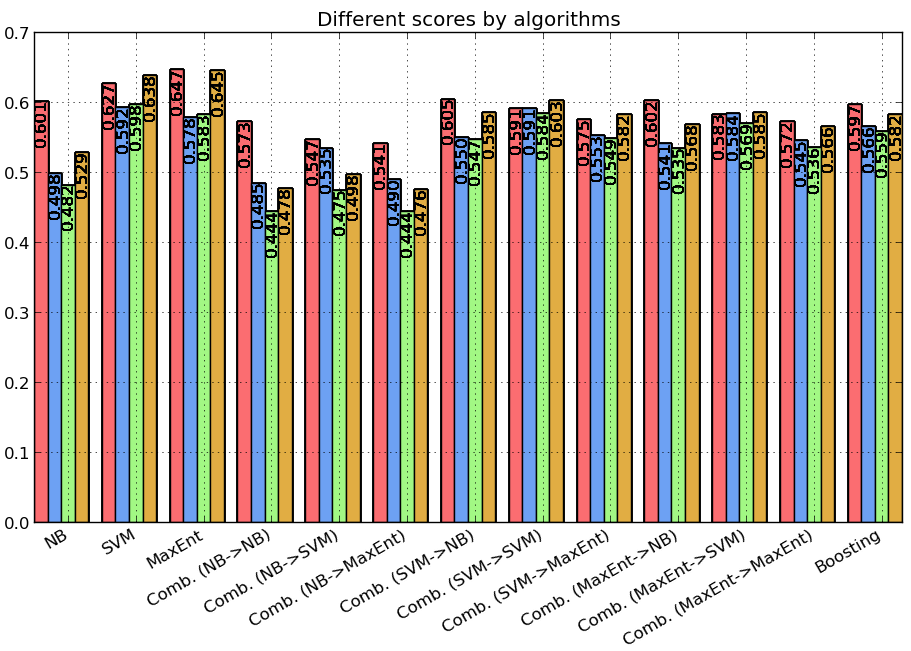
\includegraphics[width=\linewidth]{../img/plots/grid/full_biggersize.png}
 \end{center}
 \caption[Results overview across all models]{A full overview of the performance of the different models after a full grid search. Two models points out as having highest accuracies: SVM and MaxEnt. One can also see models using Naive Bayes, especially on it's own or to classify subjectivity, performs poorly.}
 \label{fig:results_full}
\end{sidewaysfigure}

As described above, an extensive grid search was conducted. This search cycled through different algorithms, parameters and preprocessing techniques. Figure~\ref{fig:results_full} displays the precision, recall, F1-score and accuracy for each of the classifiers with dev set 1 as evaluation data. We notice that most of the classifiers that involves the NB algorithm has a bad performance, both for accuracy and F1-score. This was observed for other dev sets as well. Further, we can see that the MaxEnt classifier has the best accuracy, while SVM has a slightly better F1-score.

Two-step models with SVM-based subjectivity classification exhibit the same basic behaviour. The one-step MaxEnt model classifies more tweets as neutral than the other classifiers. Using MaxEnt for subjectivity classification and either MaxEnt or SVM for polarity classification performs well, but is too heavy on the positive class. Boosting does not improve and behaves in a fashion similar to two-step MaxEnt models. All combinations involving NB tend to heavily favour positive predictions; only the two-step models involving another algorithm for polarity classification gave some improvement for negative tweets.

We can also see that all the classifiers with SVM tends to give a better confusion matrix than the others. This is shown in Figures~\ref{fig:confmat_svm} - \ref{fig:confmat_boosting}. The confusion matrices that include SVM indicates that it has a more precise classification of negative instances than the others. In tests where NB is used, the system leans much more to the positive class than the other models.

\begin{minipage}[!htb]{\linewidth}
     \centering
     \begin{minipage}{0.45\linewidth}
          \begin{figure}[H]
               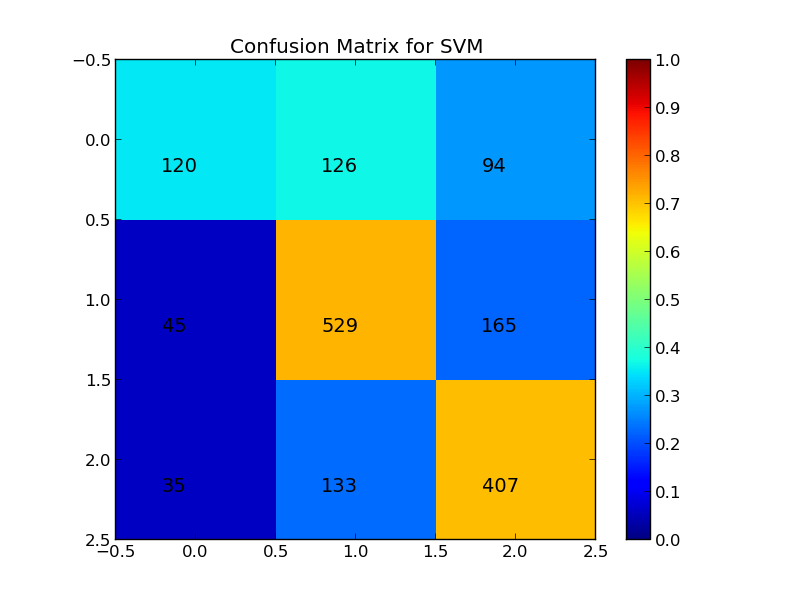
\includegraphics[width=\linewidth]{../img/plots/grid/confusion_matrix_SVM.png}
           \caption[Plot showing the confusion matrix for SVM]{Confusion matrix for the model using SVM. Performs well on both neutral and positive predictions, but somewhat poor on negative.}
           \label{fig:confmat_svm}
          \end{figure}
     \end{minipage}
     \hspace{0.05\linewidth}
     \begin{minipage}{0.45\linewidth}
          \begin{figure}[H]
               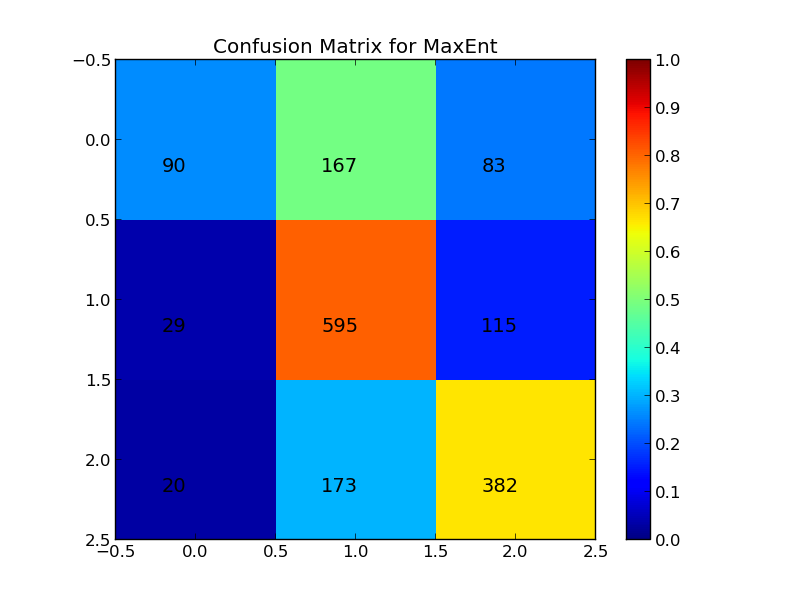
\includegraphics[width=\linewidth]{../img/plots/grid/confusion_matrix_MaxEnt.png}
           \caption[Plot showing the confusion matrix for MaxEnt]{Confusion matrix for the model using MaxEnt. Performs especially good on neutral tweets, but seem to be classifying neutral too much.}
           \label{fig:confmat_maxent}
          \end{figure}
     \end{minipage}
 \end{minipage}    
 
 \begin{minipage}[!htb]{\linewidth}
      \centering
     \begin{minipage}{0.45\linewidth}
          \begin{figure}[H]
               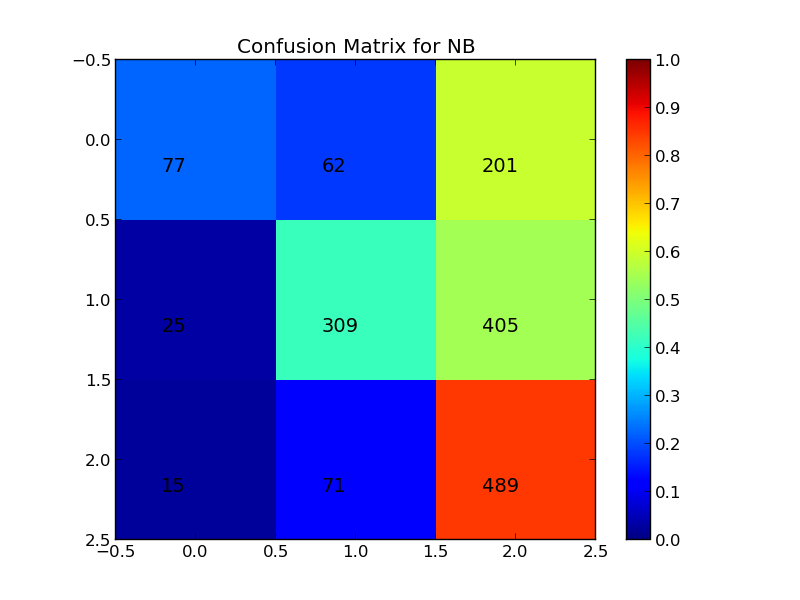
\includegraphics[width=\linewidth]{../img/plots/grid/confusion_matrix_NB.png}
           \caption[Plot showing the confusion matrix for NB]{Confusion matrix for the model using NB. Performs very well for positive tweets, but seem to favour it too much.}
           \label{fig:confmat_nb}
          \end{figure}
     \end{minipage}
     \hspace{0.05\linewidth}
     \begin{minipage}{0.45\linewidth}
          \begin{figure}[H]
               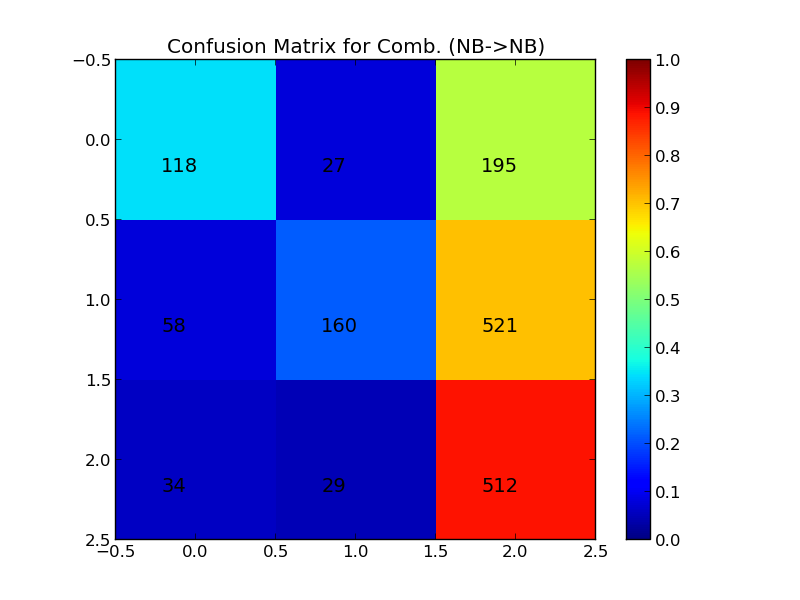
\includegraphics[width=\linewidth]{../img/plots/grid/confusion_matrix_Comb-NB-NB.png}
           \caption[Plot showing the confusion matrix for two-step NB -> NB]{Confusion matrix for the two-step model using NB for both subjectivity/objectivity and polarity classification. Shows the same trend as when using NB in a one-step model. Model favours positive predictions.}
           \label{fig:confmat_nb_nb}
          \end{figure}
     \end{minipage}
\end{minipage}

\begin{minipage}[!htb]{\linewidth}
     \centering
     \begin{minipage}{0.45\linewidth}
          \begin{figure}[H]
               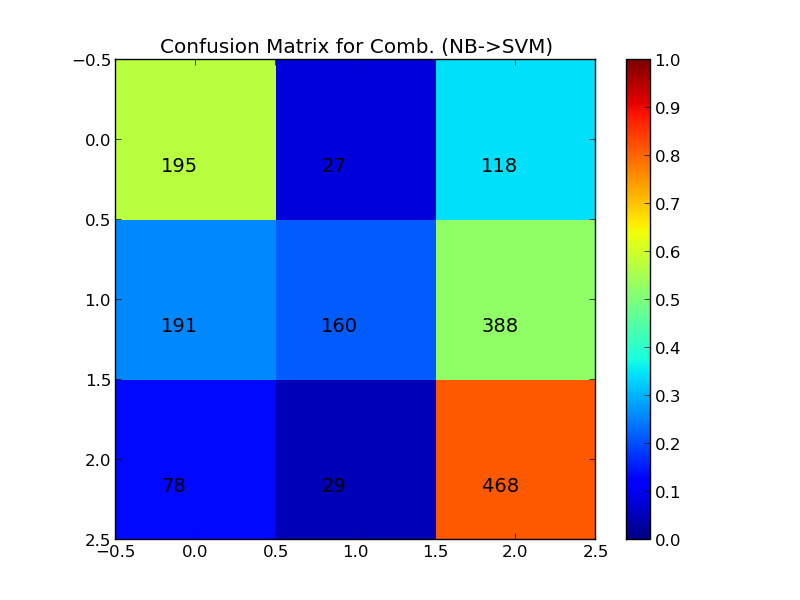
\includegraphics[width=\linewidth]{../img/plots/grid/confusion_matrix_Comb-NB-SVM.png}
           \caption[Plot showing the confusion matrix for two-step NB -> SVM]{Confusion matrix for the two-step model using NB for subjectivity/objectivity classification and SVM for polarity. Shows the same trend as when using NB in a one-step model. Model favours positive predictions but performing better for negative tweets.}
           \label{fig:confmat_nb_svm}
          \end{figure}
     \end{minipage}
     \hspace{0.05\linewidth}
     \begin{minipage}{0.45\linewidth}
          \begin{figure}[H]
               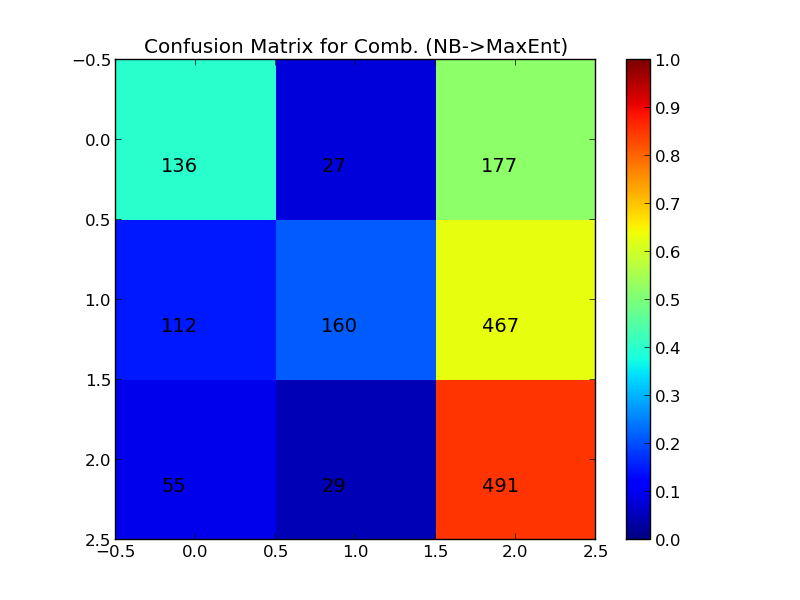
\includegraphics[width=\linewidth]{../img/plots/grid/confusion_matrix_Comb-NB-MaxEnt.png}
           \caption[Plot showing the confusion matrix for two-step NB -> MaxEnt]{Confusion matrix for the two-step model using NB for subjectivity/objectivity classification and SVM for polarity. Shows the same trend as when using the NB -> SVM model. Model favours positive predictions but performing better for negative tweets.}
           \label{fig:confmat_nb_maxent}
          \end{figure}
     \end{minipage}
\end{minipage}

\begin{minipage}[!htb]{\linewidth}
     \centering
     \begin{minipage}{0.45\linewidth}
           \begin{figure}[H]
                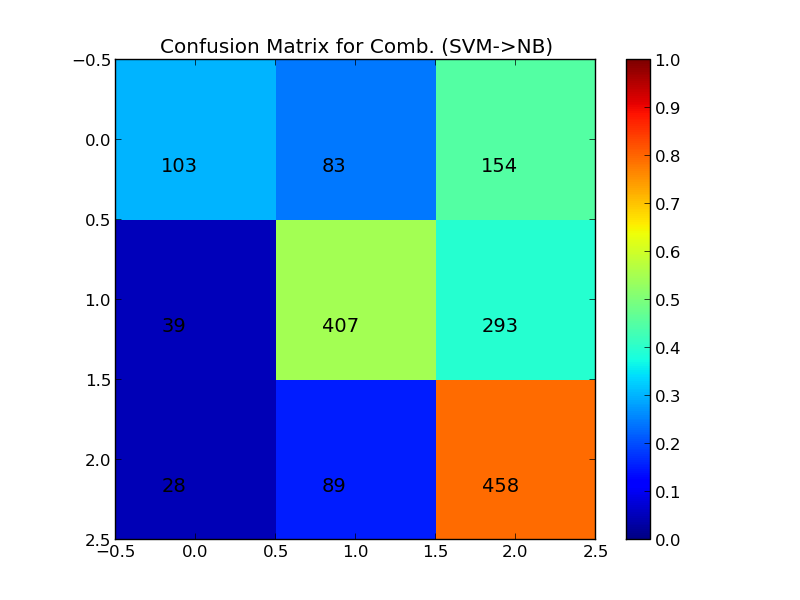
\includegraphics[width=\linewidth]{../img/plots/grid/confusion_matrix_Comb-SVM-NB.png}
        		\caption[Plot showing the confusion matrix for two-step SVM -> NB]{Confusion matrix for the model using SVM and NB. Performs good for positive tweets, but not as good for neutral and negative.}
            \label{fig:confmat_svm_nb}
           \end{figure}
      \end{minipage}
      \hspace{0.05\linewidth}
      \begin{minipage}{0.45\linewidth}
           \begin{figure}[H]
                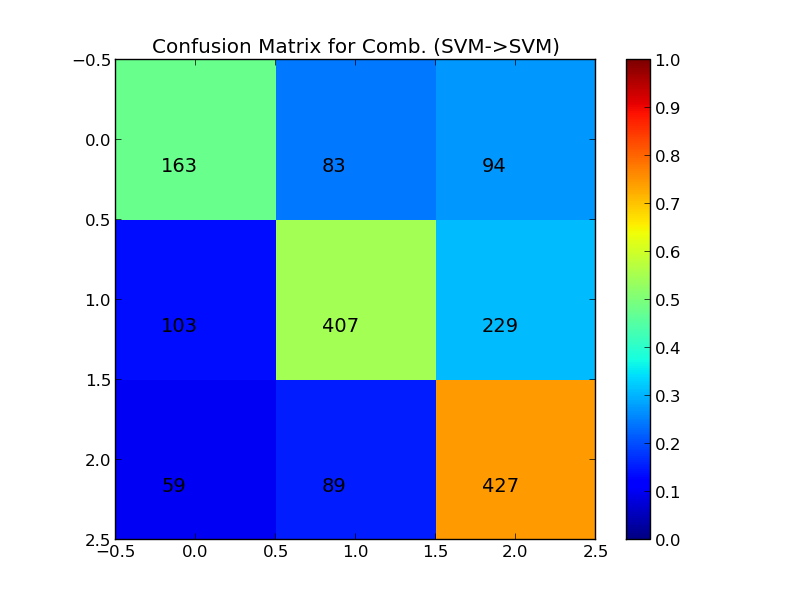
\includegraphics[width=\linewidth]{../img/plots/grid/confusion_matrix_Comb-SVM-SVM.png}
         		\caption[Plot showing the confusion matrix for two-step SVM -> SVM]{Confusion matrix for the model using SVM and SVM. Performs good across the board, and shows a good diagonal colour profile in the plot.}
            \label{fig:confmat_svm_svm}
           \end{figure}
      \end{minipage} \\
 \end{minipage}
 
 \begin{minipage}[!htb]{\linewidth}
      \centering
     \begin{minipage}{0.45\linewidth}
          \begin{figure}[H]
               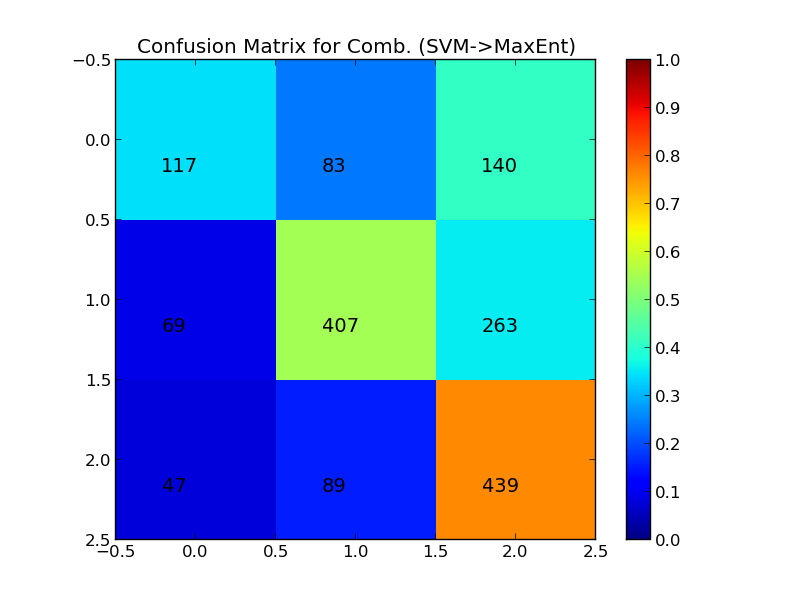
\includegraphics[width=\linewidth]{../img/plots/grid/confusion_matrix_Comb-SVM-MaxEnt.png}
           \caption[Plot showing the confusion matrix for two-step SVM -> MaxEnt]{Confusion matrix for the model using SVM and MaxEnt. Performs good for neutral and positive tweets, but not too well with negative tweets.}
           \label{fig:confmat_svm_maxent}
          \end{figure}
     \end{minipage}
     \hspace{0.05\linewidth}
     \begin{minipage}{0.45\linewidth}
          \begin{figure}[H]
               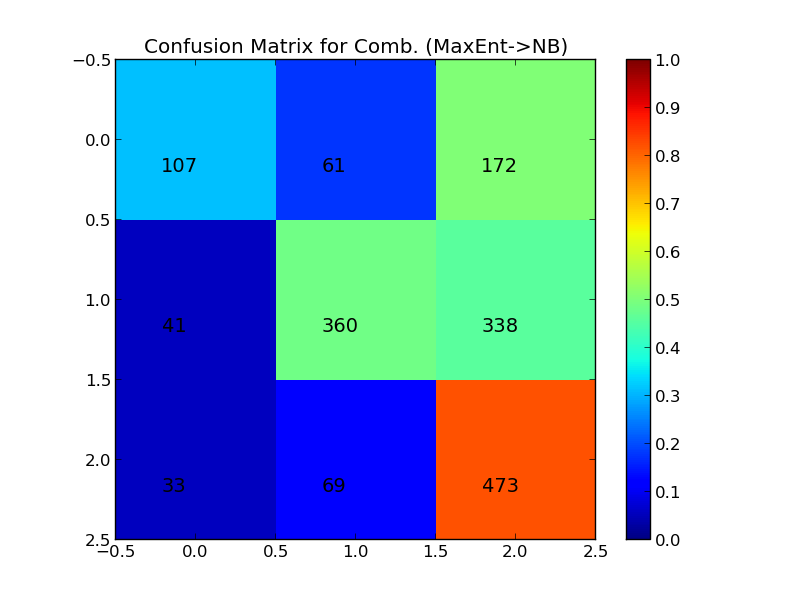
\includegraphics[width=\linewidth]{../img/plots/grid/confusion_matrix_Comb-MaxEnt-NB.png}
           \caption[Plot showing the confusion matrix for two-step MaxEnt -> NB]{Confusion matrix for the model using MaxEnt and NB. Performs good for positive tweets, but not too well with negative and neutral tweets.}
           \label{fig:confmat_maxent_nb}
          \end{figure}
     \end{minipage}
\end{minipage}
     
\begin{minipage}[htb!]{\linewidth}
     \centering
     \begin{minipage}{0.45\linewidth}
          \begin{figure}[H]
               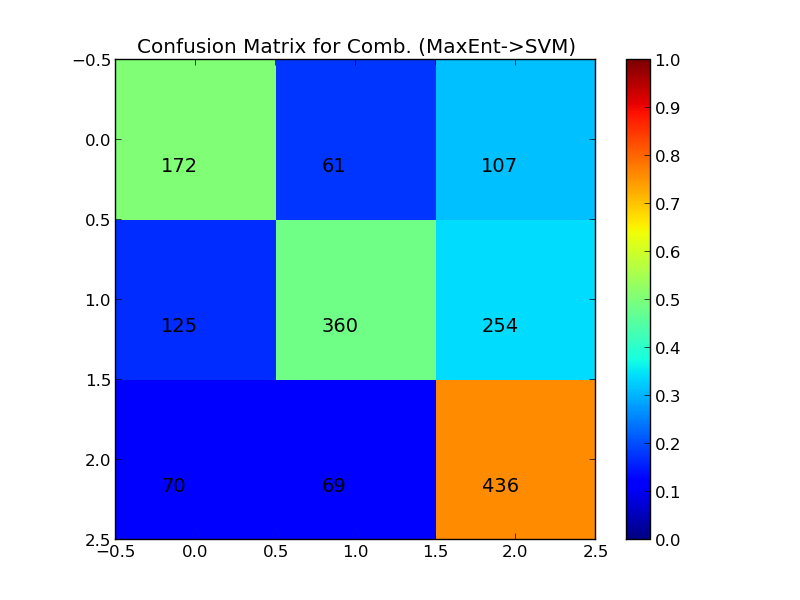
\includegraphics[width=\linewidth]{../img/plots/grid/confusion_matrix_Comb-MaxEnt-SVM.png}
           \caption[Plot showing the confusion matrix for two-step MaxEnt -> SVM]{Confusion matrix for the model using MaxEnt and SVM. Performs good but is too heavy on the positive classification.}
           \label{fig:confmat_maxent_svm}
          \end{figure}
     \end{minipage}
     \hspace{0.05\linewidth}
     \begin{minipage}{0.45\linewidth}
          \begin{figure}[H]
               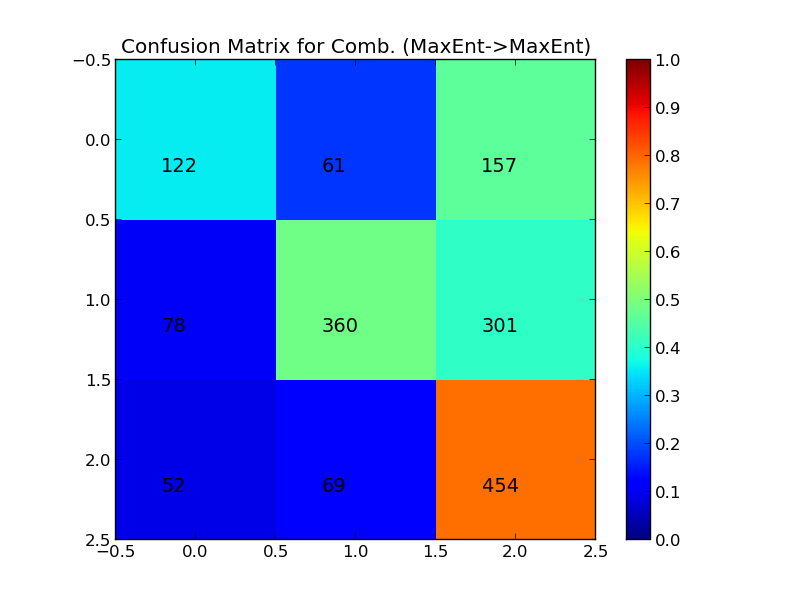
\includegraphics[width=\linewidth]{../img/plots/grid/confusion_matrix_Comb-MaxEnt-MaxEnt.png}
           \caption[Plot showing the confusion matrix for two-step MaxEnt -> MaxEnt]{Confusion matrix for the model using MaxEnt and MaxEnt. As with MaxEnt -> SVM, this model performs good but is too heavy on the positive classification.}
           \label{fig:confmat_maxent_maxent}
          \end{figure}
     \end{minipage}
\end{minipage}

\begin{minipage}[htb!]{\linewidth}
     \centering
     \begin{minipage}{0.45\linewidth}
	     \begin{figure}[H]
	          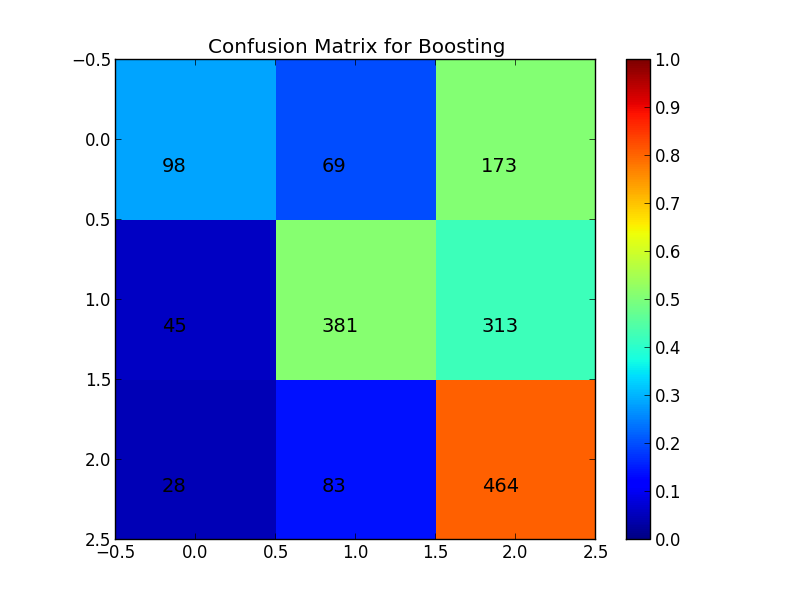
\includegraphics[width=\linewidth]{../img/plots/grid/confusion_matrix_Boosting.png}
	      \caption[Plot showing the confusion matrix for Boosting]{Confusion matrix for the model using Boosting. Showing the same trend as the MaxEnt -> SVM and MaxEnt -> MaxEnt models, tends to classify too much positive.}
	      \label{fig:confmat_boosting}
	     \end{figure}
     \end{minipage}
\end{minipage}



As a part of the grid search, the system applied all the different preprocessing methods for each classifier. Figure~\ref{fig:preprocess_usage} clearly shows that P2 (removing user names, URLs, hash-tag prefixes, RT-tokens and redundant letters. See table~\ref{tab:preproc_desc}) is the pre-processing method that was most used, i.e., it gave the best accuracy. Figure~\ref{fig:preprocess_usage} also indicates that URLs are noisy, and does not contain any sentiment, and that hash-tags and emoticons are valuable features. We can see that with the P2 pre-processing method, there is no real Twitter specific feature. The hash-tag is included, but used as a regular word.

\begin{figure}[!htb]
	\centering
	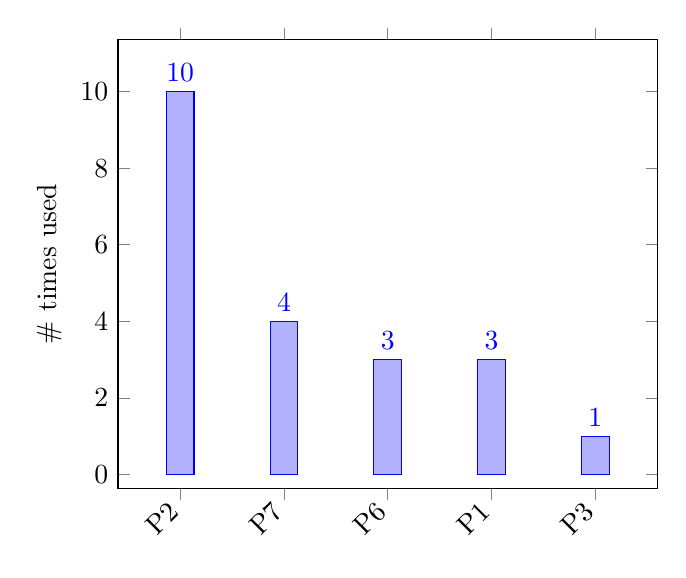
\begin{tikzpicture}
	  \begin{axis}[
	    ybar,
	    enlargelimits=0.15,
	    legend style={at={(0.5,-0.2)},
	      anchor=north,legend columns=-1},
	    ylabel={\# times used},
	    symbolic x coords={P2,P7,P6, P1,P3},
	    xtick=data,
	    nodes near coords, 
		nodes near coords align={vertical},
	    x tick label style={rotate=45,anchor=east},
	    ]
	    \addplot coordinates {(P2,10) (P7,4) 
			(P6,3) (P1,3) (P3,1)};
	  \end{axis}
	\end{tikzpicture}
	\caption[Statistics of pre-processing usage.]{Statistics of pre-processing usage. Removing all usernames, urls, hash-tag character, RT-tag and excessive letters as features seem to give best performance.}
	\label{fig:preprocess_usage}
\end{figure}

\clearpage
\subsection{SVM vs MaxEnt}

From the full grid search, the best parameters on SVM and MaxEnt was extracted and more detailed tests were done with only using SVM and MaxEnt, without grid searching. The best parameters for the SVM model, was using unigram, P2 pre-processing method, not removing stop words, and a C value of 1.0. For the MaxEnt model, the P3 pre-processing method was used, along with unigrams, IDF, not removing stop words and 0.3 as C value. Penalty for MaxEnt was selected to be L1. Full parameter selection for SVM and MaxEnt is visible in~table~\ref{tab:svm_maxent_best_params}. The SVM and MaxEnt models, with these parameters, were tested with an additional development set (dev set 2).

The results for both the SVM and MaxEnt classifiers with dev set 1 are shown in figure~\ref{fig:best_result}. With dev set 2, SVM's performance is much better than MaxEnt's, as seen in table~\ref{tab:performance}. Dev set 1 contain more neutral tweets than dev set 2, which gives us a reason to believe that it favours the MaxEnt classifier. In MaxEnt's confusion matrix from the first search, shown in Figure~\ref{fig:confmat_maxent}, we can see that it classifies more neutral tweets than the other classifiers.

\begin{table}[!htb]
\centering
\begin{tabular}{|r||c|c|c|} 
\cline{2-3}
\multicolumn{1}{c|}{ } & \textbf{SVM} & \textbf{MaxEnt} \\ \hline
ngram\_range & 1,1 & 1,1 \\ \hline
sunlinear\_tf  & True & True \\ \hline
preprocessor & P2 & P3 \\ \hline
use\_idf & True & True \\ \hline
smooth\_idf & True & True \\ \hline
max\_df & 0.5 & 0.5 \\ \hline
stop\_words & None & None \\ \hline
C & 1.0 & 0.3 \\ \hline
penalty &  & l1 \\ \hline

\end{tabular}
\caption[Selected parameters from grid search]{Table showing an overview of the selected parameters for both the SVM and MaxEnt model. Parameters selected by doing an excessive grid search.}
\label{tab:svm_maxent_best_params}
\end{table}


\begin{table}[!htb]
	\centering
	\begin{tabular}{l|cc|cc} 
	\noalign{\smallskip}\hline\noalign{\smallskip}
	Data set & \multicolumn{2}{c|}{Dev set 1} & \multicolumn{2}{c}{Dev set 2} \\
	Learner  & SVM    & MaxEnt & SVM    & MaxEnt \\
	\noalign{\smallskip}\hline\noalign{\smallskip}
	Precision  & 0.627  & {\bf 0.647}   & {\bf 0.700}  & 0.561 \\
	Recall       & {\bf 0.592}  & 0.578  & {\bf 0.726}  & 0.589 \\
	F1-score  & {\bf 0.598}  & 0.583  & {\bf 0.707}  & 0.556 \\
	Accuracy & 0.638  & {\bf 0.645}  & {\bf 0.728}  & 0.581 \\
	\noalign{\smallskip}\hline\noalign{\smallskip}
	\end{tabular}
	\caption[Best classifier performance]{Best classifier performance {\small (bold=best score)}. Shows that using dev set 1 MaxEnt has better accuracy and precision, but SVM performs better in regards to F1-score and recall. For dev set 2, SVM have higher measures across the board.}
	\label{tab:performance}
\end{table}


To even out the distribution of the different classes, we did a grid search with a reduced training set. Figure~\ref{fig:svm_reduced_1000} and~\ref{fig:svm_reduced_2000} shows SVM's results when reducing the training set to a maximum of 1000 and 2000 tweets per class. The accuracy on SVM is highest on the original training set, but the F1-score and Recall improves on reducing the training set to maximum 2000 per class. See complete effects of reducing training set in~table~\ref{tab:svm_reduced}. The negative classification improves when reducing the training set to maximum 2000 tweets per class, but the accuracy for neutral and positive tweets decrease. Similar observation can be made when reducing the data set to 1000. Negative tweets perform better, but positive and neutral performance is worse. This can be deduced from~figure~\ref{fig:best_result_confusion},~\ref{fig:svm_reduced_2000} and~\ref{fig:svm_reduced_1000}.


\begin{table}[!htb]
	\centering
	\begin{tabular}{l|ccc} 
	\noalign{\smallskip}\hline\noalign{\smallskip}
	Data size  & Original       & 2000   & 1000 \\
	\noalign{\smallskip}\hline\noalign{\smallskip}
	Precision  & {\bf 0.627}  & 0.612 & 0.570 \\
	Recall       & 0.592  & \textbf{0.618} & 0.586 \\
	F1-score  & 0.598  & \textbf{0.614} & 0.563 \\
	Accuracy & {\bf 0.639}  & 0.630 & 0.569 \\
	\noalign{\smallskip}\hline\noalign{\smallskip}
	\end{tabular}
	\caption{Effects on SVM trained with reduced training sets}
	\label{tab:svm_reduced}
\end{table}


\begin{table}[!htb]
	\centering
	\begin{tabular}{|c|c|c|c|}
	
		\multicolumn{4}{c}{SVM} \\ \hline
		
		\# & Negative & Neutral & Positive \\ \hline\hline
		
		1 & no  		& wear & wait \\ \hline
		2 & didn't  	& tallahassee & nice \\ \hline
		3 & cancelled  	& 15th & interesting \\ \hline
		4 & don't  		& 26 & awesome \\ \hline
		5 & worse  		& at & cool \\ \hline
		6 & why  		& trip & amazing \\ \hline
		7 & bad  		& joe & fun \\ \hline
		8 & worst  		& theres & ! \\ \hline
		9 & hate  		& arrows & :) \\ \hline
		10 & shit  		& murphy, & excited \\ \hline
		11 & sad  		& question & happy \\ \hline
		12 & sorry  		& plan & love \\ \hline
		13 & not  		& set & best \\ \hline
		14 & fuck  		& 8th & great \\ \hline
		15 & :(  		& paterno & good \\ \hline
	\end{tabular}
	
	\caption[Most informative features for SVM]{Top 15 of the most informative features for SVM}
	\label{tab:informative_features_svm}
\end{table}


\begin{table}[!htb]
	\centering
	\begin{tabular}{|c|c|c|c|}		
	\multicolumn{4}{c}{MaxEnt} \\ \hline
	
	\# & Negative & Neutral & Positive \\ \hline\hline
	
	1 & no 	& center & glad \\ \hline
	2 & don't 	& royal & nice \\ \hline
	3 & why 	& plan & thanks \\ \hline
	4 & bad 	& joe & cool \\ \hline
	5 & shit 	& nov & awesome \\ \hline
	6 & injury 	& george & interesting \\ \hline
	7 & cancelled 	& theres & amazing \\ \hline
	8 & hate 	& arrows & :) \\ \hline
	9 & worst 	& trip & fun \\ \hline
	10 & worse 	& set & best \\ \hline
	11 & fuck 	& question & excited \\ \hline
	12 & sorry 	& at & love \\ \hline
	13 & not 	& url & happy \\ \hline
	14 & sad 	& 8th & good \\ \hline
	15 & :( 	& paterno & great \\ \hline
	\end{tabular}
	
	\caption[Most informative features]{Top 15 of the most informative features for MaxEnt}
	\label{tab:informative_features_maxent}
\end{table}


The features in tables~\ref{tab:informative_features_svm} and~Table~\ref{tab:informative_features_maxent}  is the most informative features from each of the classifiers in the second grid search. Some features are represented among the top 15 for both SVM and MaxEnt, and most of these features makes sense. As we did not normalize the features, we can see that some words appears in different forms and degrees (e.g., "worse", "worst" and "don't", "didn't"). For both MaxEnt and SVM, emoticons are listed among the most informative features. In the case of SVM, the exclamation point is an informative feature for positive classification.

We see that for the most part the features seem to make sense, but we see some anomalies. Both SVM and MaxEnt show 'why' as a negative feature, which is normally incorrect. In addition, the most informative feature for SVM is wait, which is not a particularly positively charged word.


\begin{figure}[!htb]
	\centering
	\begin{minipage}{.45\linewidth}
		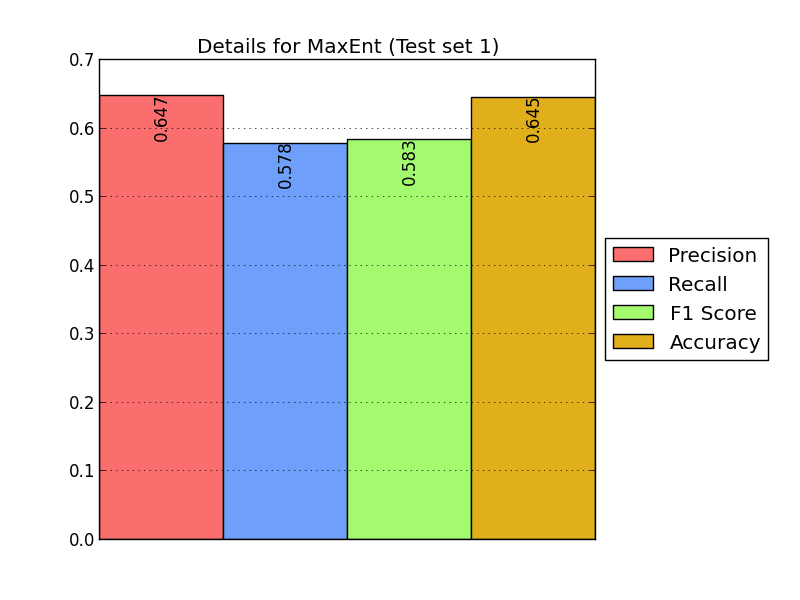
\includegraphics[width=\linewidth]{../img/plots/analysis/maxent_stats_best.png}
	\end{minipage}
	\hspace{0.05\linewidth}
	\begin{minipage}{.45\linewidth}
		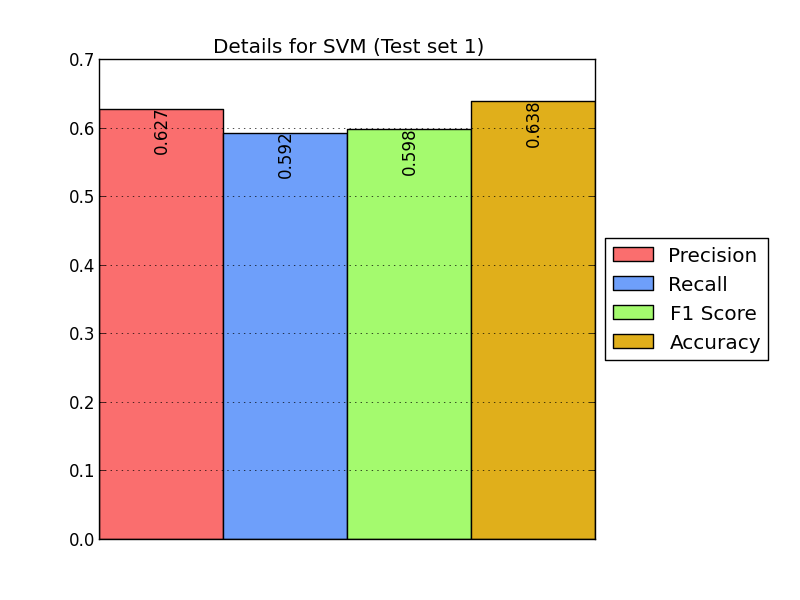
\includegraphics[width=\linewidth]{../img/plots/analysis/svm_stats_best.png}
	\end{minipage}
	\caption[Best performance plots for SVM and MaxEnt]{Best performance plots for SVM and MaxEnt. We see that MaxEnt has better Precision and Accuracy, but SVM scores higher on F1-score and Recall.}
	\label{fig:best_result}
\end{figure}

\begin{figure}[!htb]
	\centering
	\begin{minipage}{.45\linewidth}
		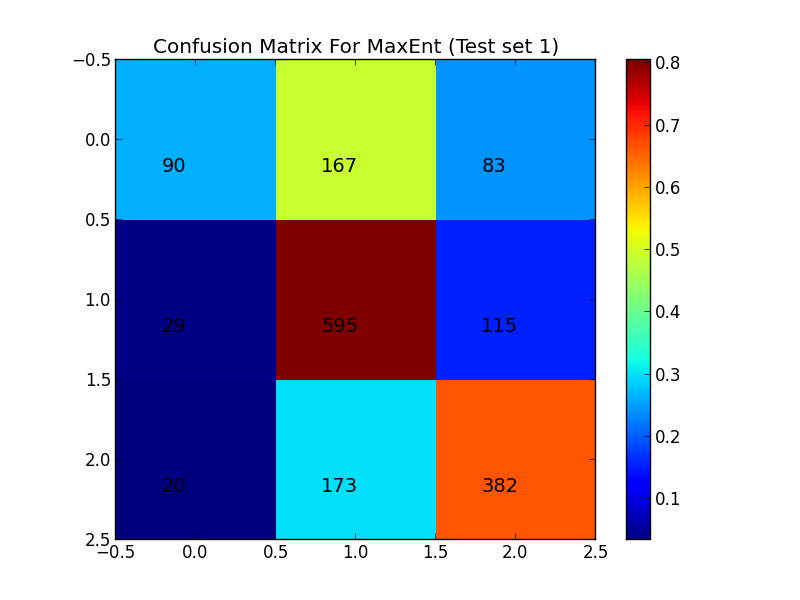
\includegraphics[width=\linewidth]{../img/plots/analysis/maxent_confusion_matrix_best.png}
	\end{minipage}
	\hspace{0.05\linewidth}
	\begin{minipage}{.45\linewidth}
		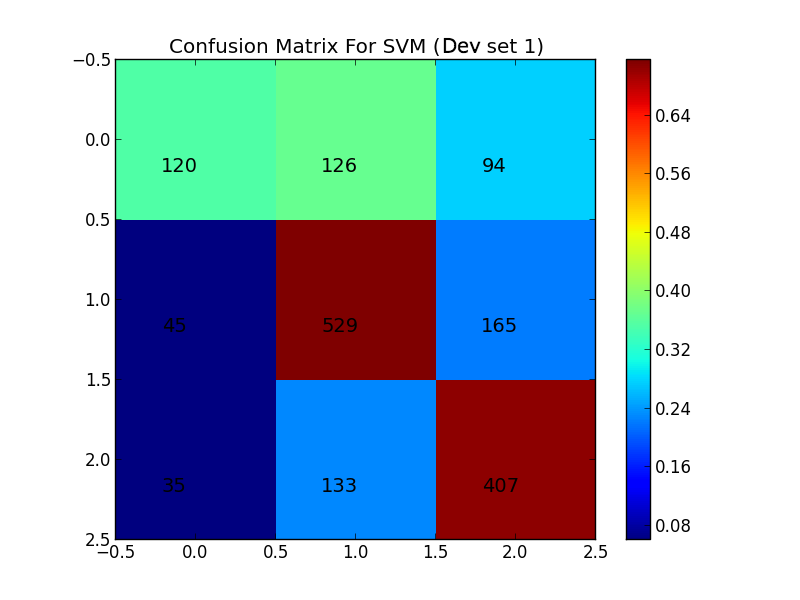
\includegraphics[width=\linewidth]{../img/plots/analysis/svm_confusion_matrix_best.png}
	\end{minipage}
	\caption[Confusion Matrix for SVM and MaxEnt]{Confusion Matrix for SVM and MaxEnt. MaxEnt favours neutral classification, and perfoms poorer than SVM on both positive and negative classifications.}
	\label{fig:best_result_confusion}
\end{figure}

\begin{figure}[!htb]
	\centering
	\begin{minipage}{.45\linewidth}
		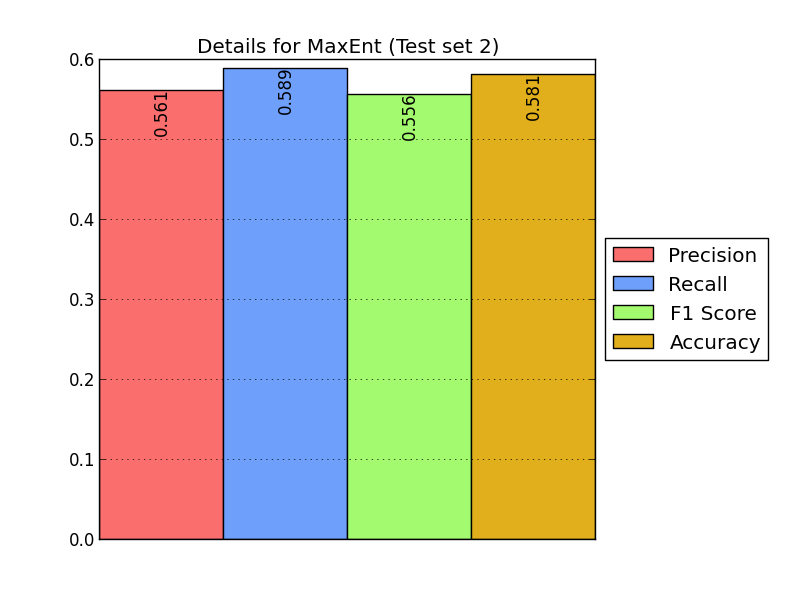
\includegraphics[width=\linewidth]{../img/plots/analysis/maxent_stats_best_diff_test.png}
	\end{minipage}
	\hspace{0.05\linewidth}
	\begin{minipage}{.45\linewidth}
		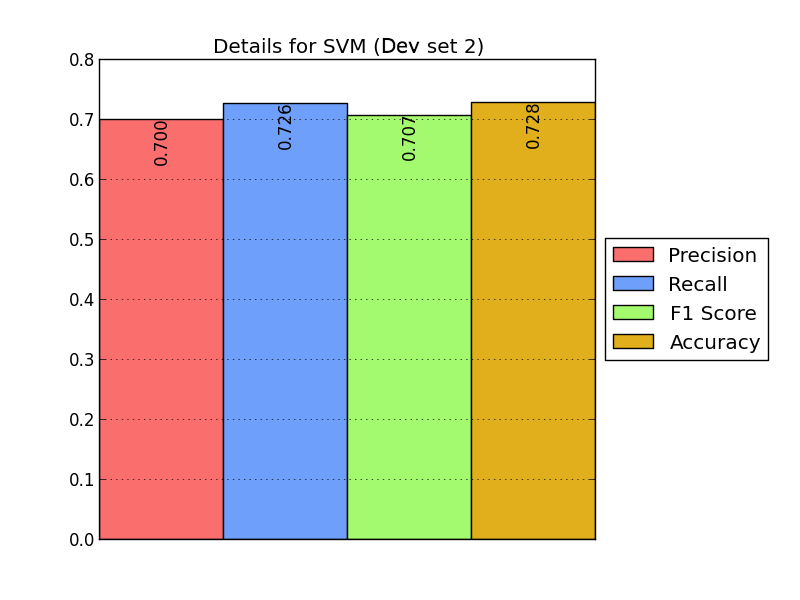
\includegraphics[width=\linewidth]{../img/plots/analysis/svm_stats_best_diff_test.png}
	\end{minipage}
	\caption[Best performance plots for SVM and MaxEnt for dev set 2]{Best performance plots for SVM and MaxEnt using dev set 2. SVM outperforms MaxEnt with \textbf{0.728} in accuracy versus \textbf{0.581}. SVM performs better on all values.}
	\label{fig:best_result_testset2}
\end{figure}

\begin{figure}[!htb]
	\centering
	\begin{minipage}{.45\linewidth}
		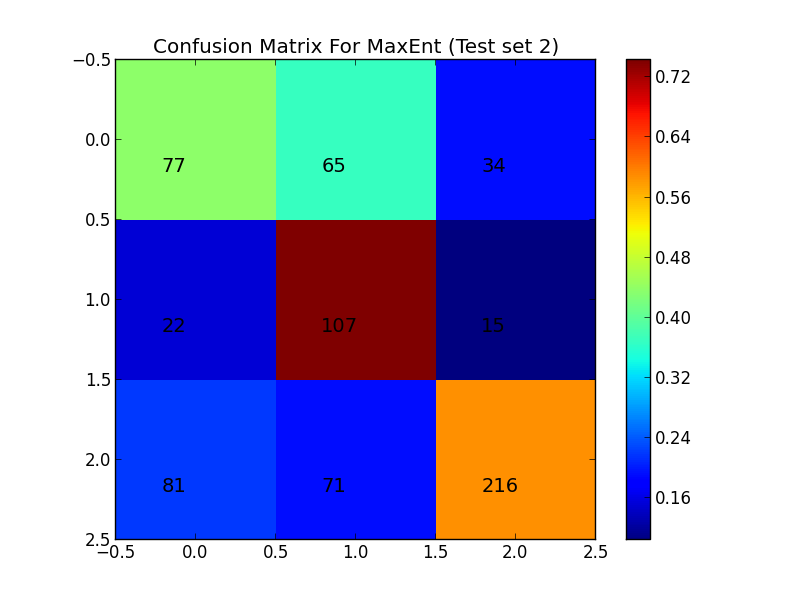
\includegraphics[width=\linewidth]{../img/plots/analysis/maxent_confusion_matrix_best_diff_test.png}
	\end{minipage}
	\hspace{0.05\linewidth}
	\begin{minipage}{.45\linewidth}
		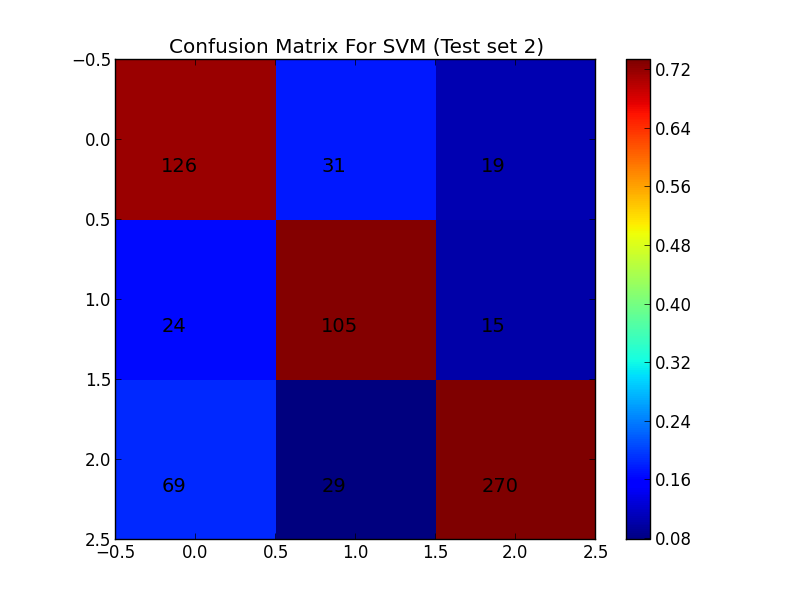
\includegraphics[width=\linewidth]{../img/plots/analysis/svm_confusion_matrix_best_diff_test.png}
	\end{minipage}
	\caption[Confusion Matrix for MaxEnt and SVM using dev set 2]{Confusion Matrix for MaxEnt and  using dev set 2. The performance difference between SVM and MaxEnt is visible in the confusion matrices as well. SVM shows a solid diagonal colour.}
	\label{fig:best_result_confusion_testset2}
\end{figure}

\begin{figure}[!htb]
	\centering
	\begin{minipage}{.45\linewidth}
		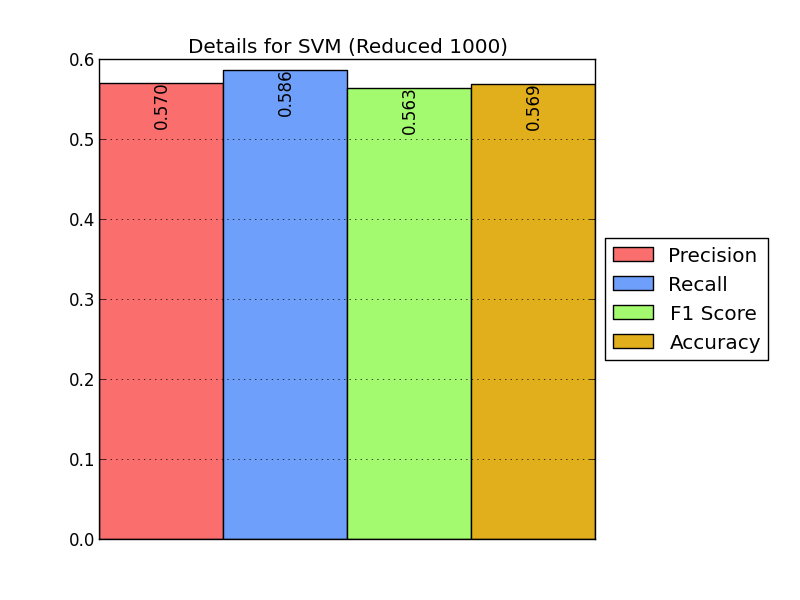
\includegraphics[width=\linewidth]{../img/plots/analysis/svm_stats_best_reduced_1000.png}
	\end{minipage}
	\hspace{0.05\linewidth}
	\begin{minipage}{.45\linewidth}
		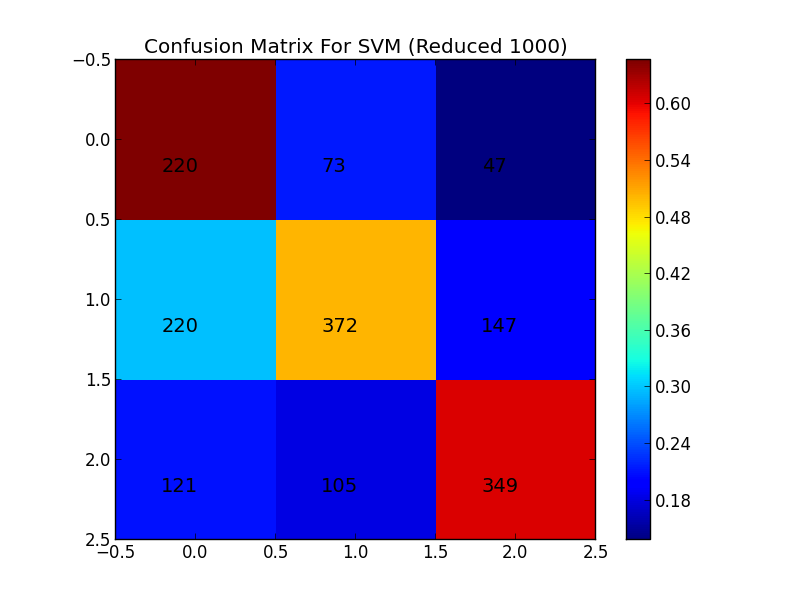
\includegraphics[width=\linewidth]{../img/plots/analysis/svm_confusion_matrix_best_reduced_1000.png}
	\end{minipage}
	\caption[Performance of SVM when reduced dataset to max 1000 per class]{Performance of SVM when reduced dataset to maximum 1000 per class. Showing better performance on negative tweets, but worse on neutral and positive. Performance generally poorer than without reduction.}
	\label{fig:svm_reduced_1000}
\end{figure}

\begin{figure}[!htb]
	\centering
	\begin{minipage}{.45\linewidth}
		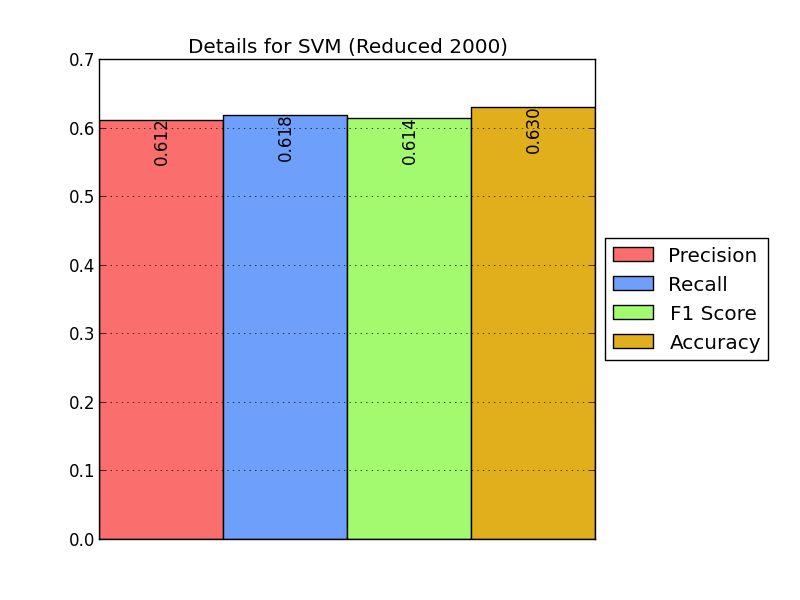
\includegraphics[width=\linewidth]{../img/plots/analysis/svm_stats_best_reduced_2000.png}
	\end{minipage}
	\hspace{0.05\linewidth}
	\begin{minipage}{.45\linewidth}
		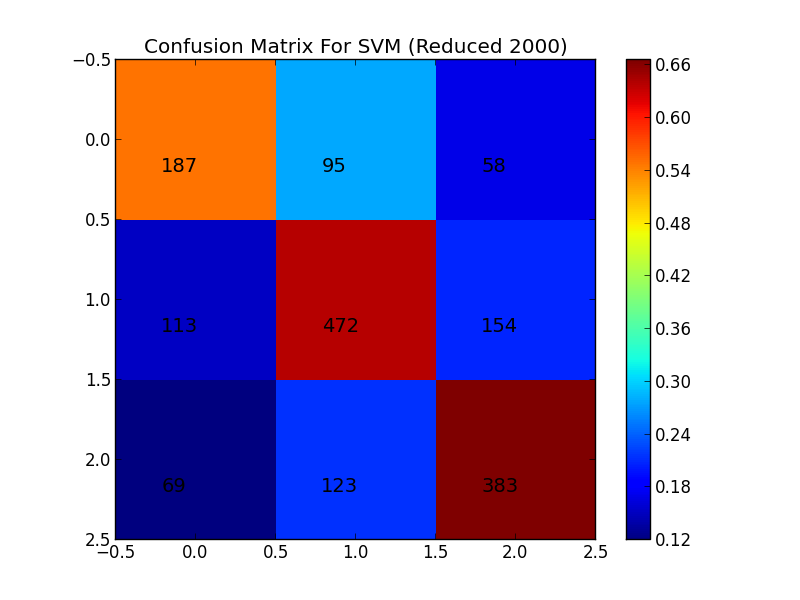
\includegraphics[width=\linewidth]{../img/plots/analysis/svm_confusion_matrix_best_reduced_2000.png}
	\end{minipage}
	\caption[Performance of SVM when reduced dataset to max 2000 per class]{Performance of SVM when reduced dataset to maximum 2000 per class. Showing better recall and F1-Score than without reduction, but poorer accuracy and precision. Some better performance on negative tweets, but poorer on neutral and positive.}
	\label{fig:svm_reduced_2000}
\end{figure}

\clearpage
\subsection{SemEval'13 Results}

Based on the information from the grid search, two systems were built for SemEval'13. Since one-step SVM-based classification showed the best performance on the training data, it was chosen for the system participating in the constrained subtask, NTNUC. The pre-processing was also the one with the best performance on the provided data, P2 which involves lower-casing all letters; reducing letter duplicates; using hash-tags as words (removing \#); and removing all URLs, user names and RT -tags.

\begin{table}

\centering
\begin{tabular}{l|cc|cc} 
\noalign{\smallskip}\hline\noalign{\smallskip}
	& \multicolumn{2}{c|}{Twitter}	& \multicolumn{2}{c}{SMS} \\
 \multicolumn{1}{r|}{\bf NTNU-}	&  {\footnotesize NTNUC}	& {\footnotesize NTNUU}	& {\footnotesize NTNUC}	& {\footnotesize NTNUU} \\
\noalign{\smallskip}\hline\noalign{\smallskip}
Precision    				& {\bf 0.652}	& 0.633 	& {\bf 0.659} 	& 0.623 \\
Recall       				& {\bf 0.579}  	& 0.564 	& {\bf 0.646} 	& 0.623  \\
F1-score  				& {\bf 0.590}  	& 0.572 	& {\bf 0.652} 	& 0.623  \\
F1 pos/neg 				& {\bf 0.532}  	& 0.507 	& {\bf 0.580} 	& 0.546  \\
\noalign{\smallskip}\hline\noalign{\smallskip}
\end{tabular}

\caption{{\bf NTNUC} and {\bf NTNUU} in SemEval'13}
\label{tab:semeval_results}
\end{table}

Given the small size of the in-house ('NTNU') data set, no major improvement was expected from adding it in the unconstrained task. Instead, a radically different set-up was chosen to create a new system, and train it on both the in-house and provided data. NTNUU utilizes a two-step approach, with SVM for subjectivity and MaxEnt for polarity classification, a combination intended to capture the strengths of both algorithms. No preprocessing was used for the subjectivity step, but user names were removed before attempting polarity classification.

As further described by~\citet{WilsonEA:13}, the SemEval'13 shared task involved testing on a set of 3813 tweets (1572 positive, 601 negative, and 1640 neutral). In order to evaluate classification performance on data of roughly the same length and type, but from a different domain, the evaluation data also included 2094 Short Message Service texts (SMS; 492 positive, 394 negative, and 1208 neutral).

Table \ref{tab:semeval_results}~shows the results obtained by the NTNU systems on the SemEval'13 evaluation data, in terms of average precision, recall and F-score for all three classes, as well as average F-score for positive and negative tweets only (F1 + / \textendash; i.e., the measure used to rank the systems participating in the shared task).
